\documentclass[9.5pt]{beamer}
%\usepackage[english]{babel}
\usepackage{fontspec}
\usepackage{hyperref}
\usepackage{animate}
\usepackage{caption}
\usepackage{amsmath}
\usepackage{graphicx}
\usepackage{amsfonts}

\usetheme{metropolis}

\metroset{numbering=none}
\metroset{block=fill}

\title{Research Project}
\subtitle{Statistical Foundations of Machine Learning}
\author{Ward Gauderis \& Fabian Denoodt}
\date{27/06/2022}
\institute{Vrije Universiteit Brussel}


\captionsetup{labelformat=empty}
\setlength\belowcaptionskip{0pt}
\captionsetup{labelfont=scriptsize,labelformat=empty}

\setlength{\fboxsep}{0pt}

\begin{document}
    \maketitle

    \begin{frame}{Summary}
        \setbeamertemplate{section in toc}[sections numbered]
        \tableofcontents
    \end{frame}


    \section{Stochastic noise and weight decay regularisation}
    \begin{frame}
        \textbf{What is the influence of stochastic noise in the dataset on the in- and out-of-sample error of a neural network and how does weight decay regularisation counter this?}
    \end{frame}

    \begin{frame}{The datasets}
        Synthetic normalised $(x, y)$ with $x \in \mathbb{R}^2, y \in \{0, 1\}$

        Controllable stochastic noise:
        \begin{itemize}
            \item \textbf{Data noise}: $x' = x + \epsilon$ with $\epsilon \sim \mathbb{N}(0, \sigma^2)$
            \item \textbf{Label noise}: swap fraction $\alpha$ of labels $y$
        \end{itemize}

        No confounding deterministic noise

        \begin{columns}[onlytextwidth]
            \column{0.5\textwidth}
            \begin{figure}
                \centering
                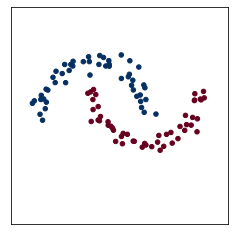
\includegraphics[width=0.7\linewidth]{images/moons}
            \end{figure}
            \column{0.5\textwidth}
            \begin{figure}
                \centering
                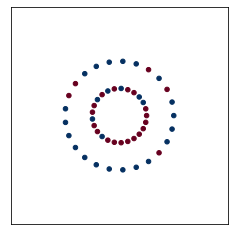
\includegraphics[width=0.7\linewidth]{images/circles}
            \end{figure}
        \end{columns}
    \end{frame}

    \begin{frame}{The models}
        \begin{block}{Neural network}
            \small
            \begin{itemize}
                \item Predict $h(x) = P(y = 1 | x)$
                \item Linear transformations with non-linear differentiable ReLU activation functions
                \item Maximise likelihood by minimising the cross-entropy error
                \item $(20, 20)$ hidden layers \& 2000 epochs
            \end{itemize}
        \end{block}

        Augmented error regularisation:
        \[E_{aug}(h, \lambda, \Omega) = E_{in}(h) + \dfrac{\lambda}{N}\Omega(h)\]

        Weight-decay with $L_2$ norm:
        \[E_{aug}(w) = E_{in}(w) + \dfrac{\lambda}{N} ||w||^2\]
    \end{frame}

    \begin{frame}{Experimental setup}
        Repeat for every combination of dataset type, label and data noise:
        \begin{enumerate}
            \item Generate 13 datasets of size 100 with noise $\in [0, 0.75]$
            \item Create 13 models of with regularisation $\in [0, 1.5]$
            \item Train every model on every dataset
            \item Compare decision boundaries and training and testing accuracies
        \end{enumerate}
    \end{frame}

    \begin{frame}{}
        \bigskip
        \begin{figure}
            \centering
            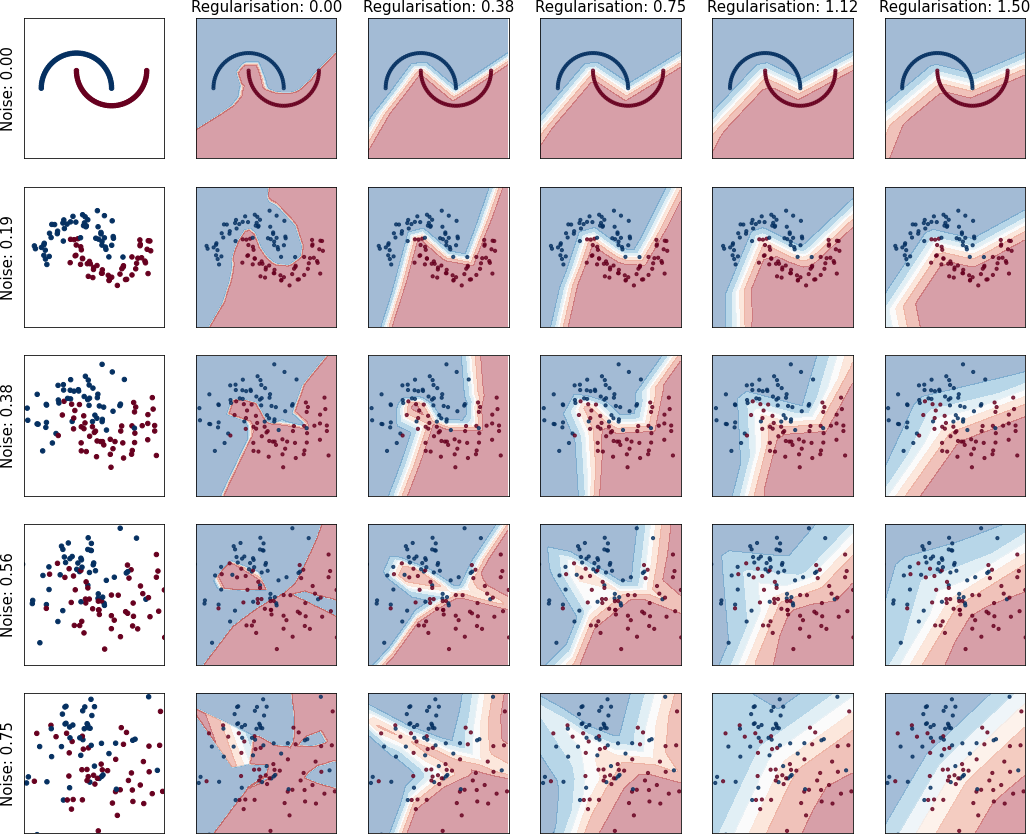
\includegraphics[height=0.9\textheight]{images/boundaries}
            \caption{Moon dataset with data noise}
        \end{figure}
    \end{frame}
    \begin{frame}{}
        \bigskip
        \begin{figure}
            \centering
            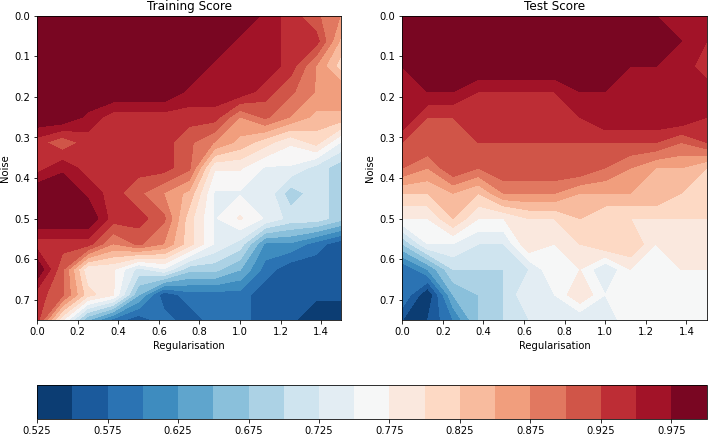
\includegraphics[width=\linewidth]{images/moon_data}
            \caption{Moon dataset with data noise}
        \end{figure}
    \end{frame}
    \begin{frame}{}
        \bigskip
        \begin{figure}
            \centering
            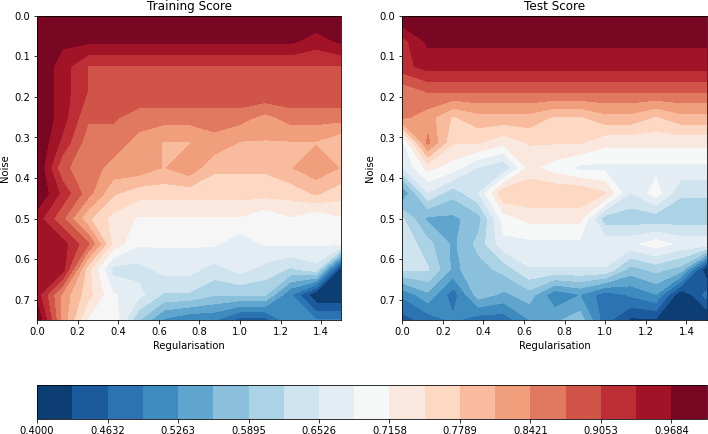
\includegraphics[width=\linewidth]{images/circles_label}
            \caption{Circles dataset with label noise}
        \end{figure}
    \end{frame}
    \begin{frame}{}
        \bigskip
        \begin{figure}
            \centering
            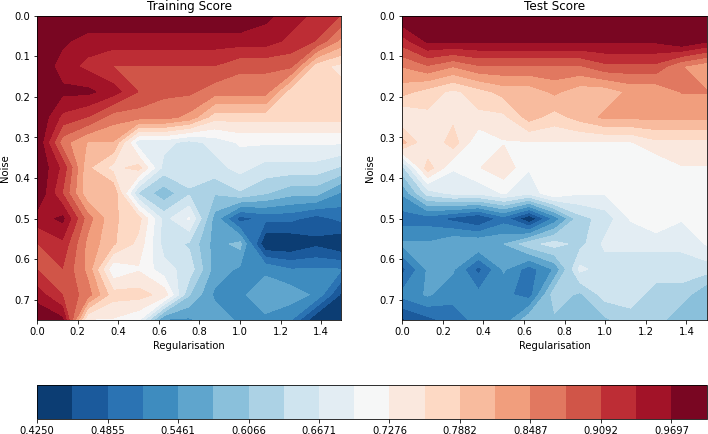
\includegraphics[width=\linewidth]{images/moon_combined}
            \caption{Moon dataset with combined noise}
        \end{figure}
    \end{frame}

    \begin{frame}{Conclusions}
        \begin{itemize}
            \item Neural networks with less effective parameters generalise better on noisier datasets

            \item Label noise versus data noise
            \begin{itemize}
                \item[-] more detrimental to generalisability
                \item[-] can be combated with less regularisation
            \end{itemize}

            \item Underfitting is less punishing than overfitting

            \item $E_{in}$ becomes less informative about $E_{out}$ with increasing noise and regularisation

            \item Optimal $\lambda$ is hard to know up front without data snooping and should be chosen through model selection
        \end{itemize}
    \end{frame}


    \section{Support vector machine kernel comparison}

    \begin{frame}
        \textbf{How do the linear kernel, polynomial kernel and radial basis function compare to each other, when applied to a synthetic two-dimensional dataset?}
    \end{frame}


    \begin{frame}{Why do we even need kernels?}
        \begin{columns}[onlytextwidth]
            \column{0.45\textwidth}
            \begin{figure}
                \centering
                \fbox{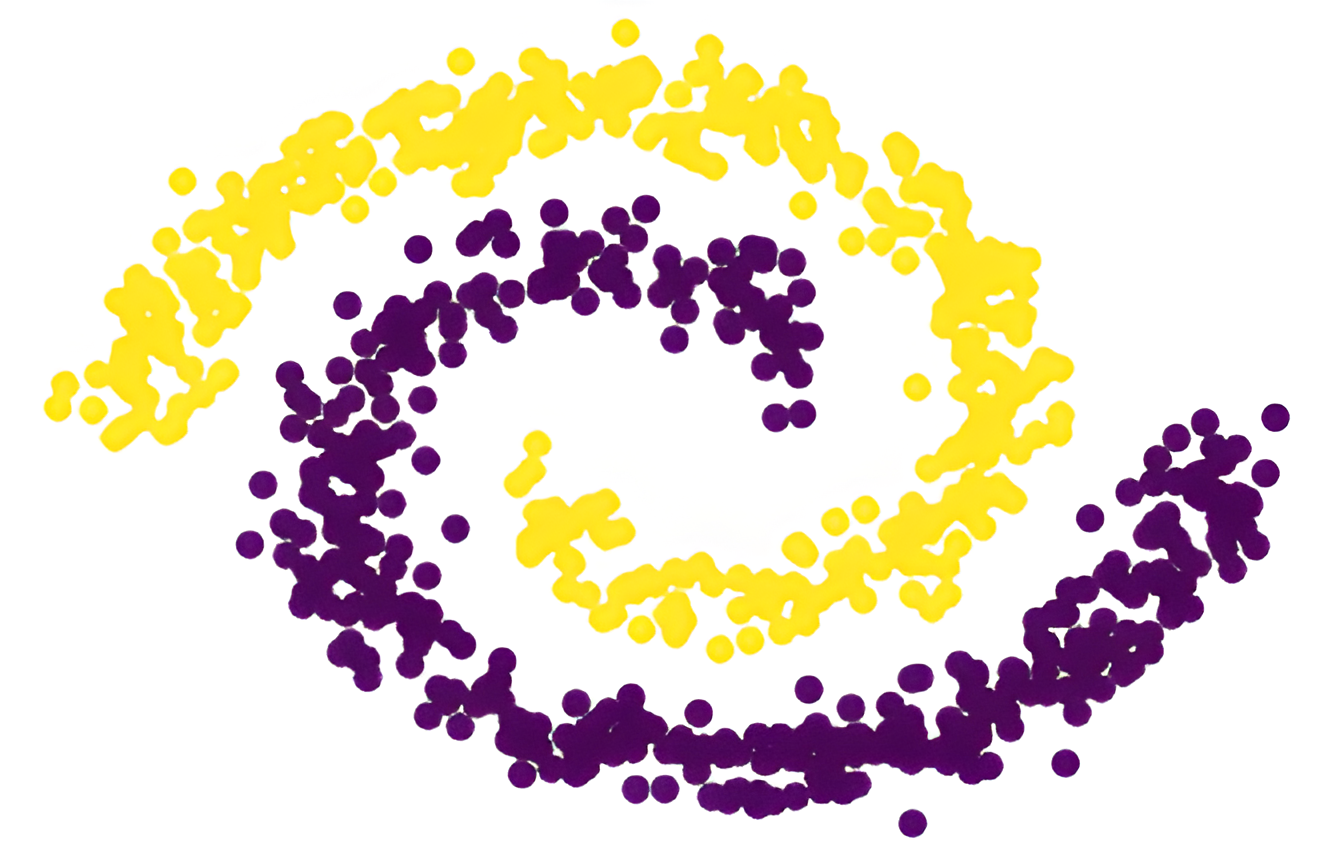
\includegraphics[width=\linewidth]{images/before}}
            \end{figure}
            \column{0.1\textwidth}
            \LARGE
            \[\mathbf{\xrightarrow{\phi}}\]
            \column{0.45\textwidth}
            \begin{figure}
                \centering
                \fbox{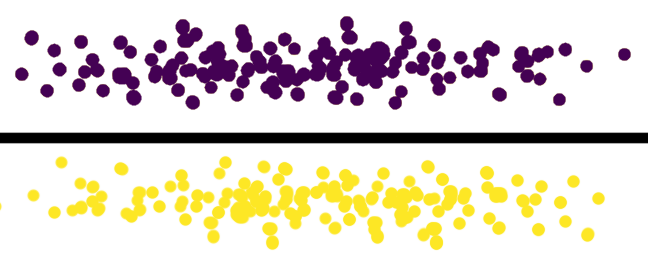
\includegraphics[width=\linewidth]{images/after}}
            \end{figure}
        \end{columns}
        \bigskip
        \begin{columns}[onlytextwidth]
            \column{0.45\textwidth}
            \tiny
            \[\mathcal{L}(\mathbf{\alpha}) = \sum_{n=1}^{N} \alpha_n-\frac{1}{2}\sum_{n=1}^{N}\sum_{m=1}^{N} y_ny_m\alpha_n\alpha_m\mathbf{x_n}^T \mathbf{x}_m\]
            \column{0.45\textwidth}
            \tiny
            \[\mathcal{L}(\mathbf{\alpha}) = \sum_{n=1}^{N} \alpha_n-\frac{1}{2}\sum_{n=1}^{N}\sum_{m=1}^{N} y_ny_m\alpha_n\alpha_m\Phi(\mathbf{x_n})^T \Phi( \mathbf{x}_m)\]
        \end{columns}
    \end{frame}
    \begin{frame}{Why do we even need kernels?}
        \begin{columns}[onlytextwidth]
            \column{0.45\textwidth}
            \begin{figure}
                \centering
                \fbox{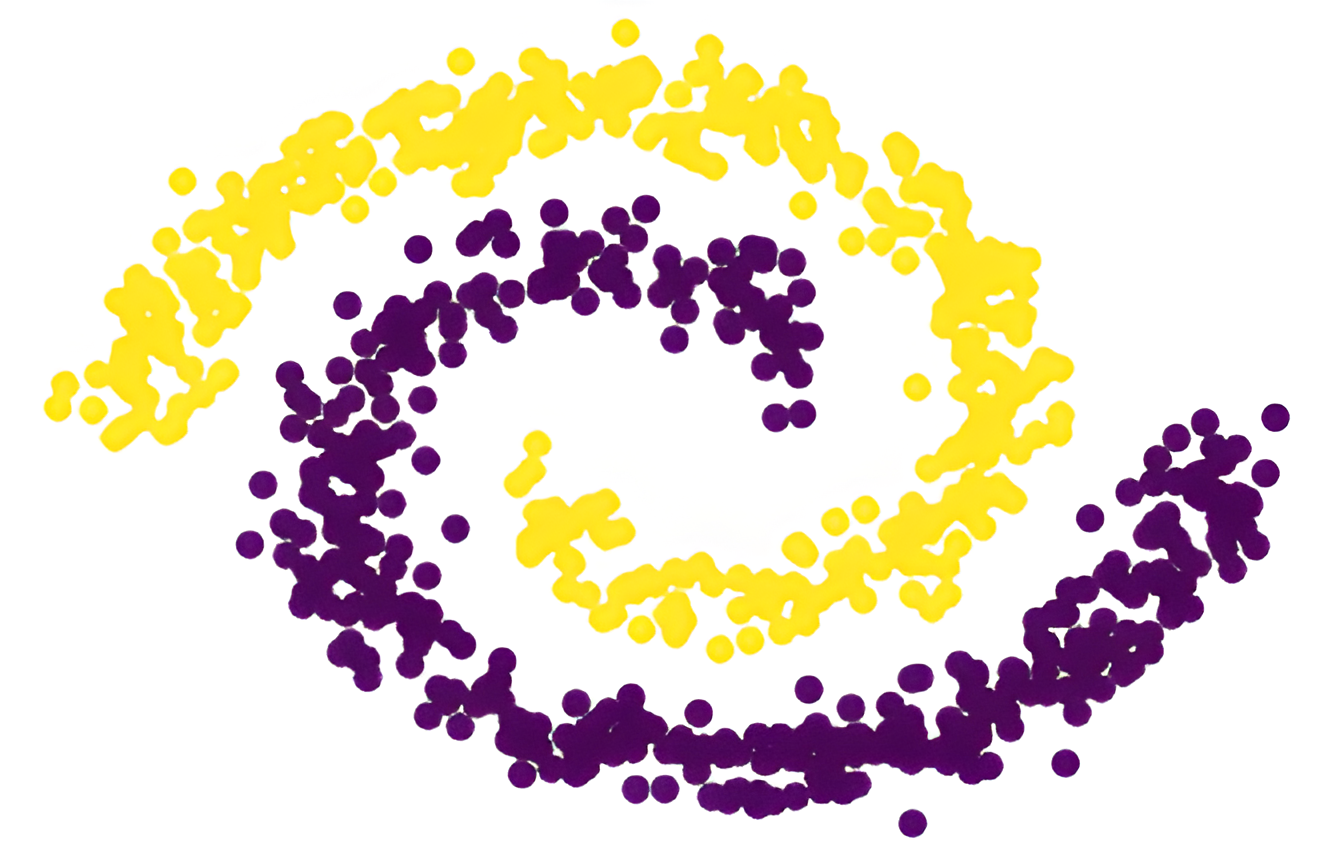
\includegraphics[width=\linewidth]{images/before}}
            \end{figure}
            \column{0.1\textwidth}
            \LARGE
            \[\mathbf{\xrightarrow{\phi}}\]
            \column{0.45\textwidth}
            \begin{figure}
                \centering
                \fbox{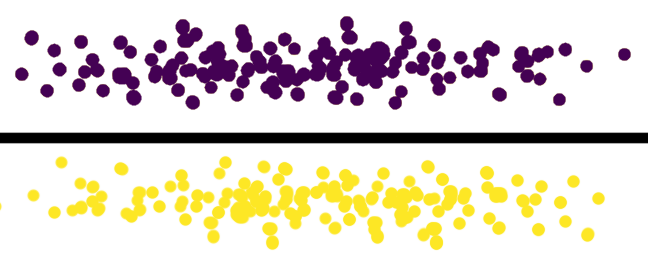
\includegraphics[width=\linewidth]{images/after}}
            \end{figure}
        \end{columns}
        \bigskip
        \begin{columns}[onlytextwidth]
            \column{0.45\textwidth}
            \tiny
            \[\mathcal{L}(\mathbf{\alpha}) = \sum_{n=1}^{N} \alpha_n-\frac{1}{2}\sum_{n=1}^{N}\sum_{m=1}^{N} y_ny_m\alpha_n\alpha_m\mathbf{x_n}^T \mathbf{x}_m\]
            \column{0.45\textwidth}
            \tiny
            \[\mathcal{L}(\mathbf{\alpha}) = \sum_{n=1}^{N} \alpha_n-\frac{1}{2}\sum_{n=1}^{N}\sum_{m=1}^{N} y_ny_m\alpha_n\alpha_m K( \mathbf{x_n} , \mathbf{x}_m)\]
        \end{columns}
    \end{frame}

    \begin{frame}[fragile]{Setup}
        \begin{columns}[onlytextwidth]
            \column{0.27\textwidth}
            \begin{figure}
                \centering
                \fbox{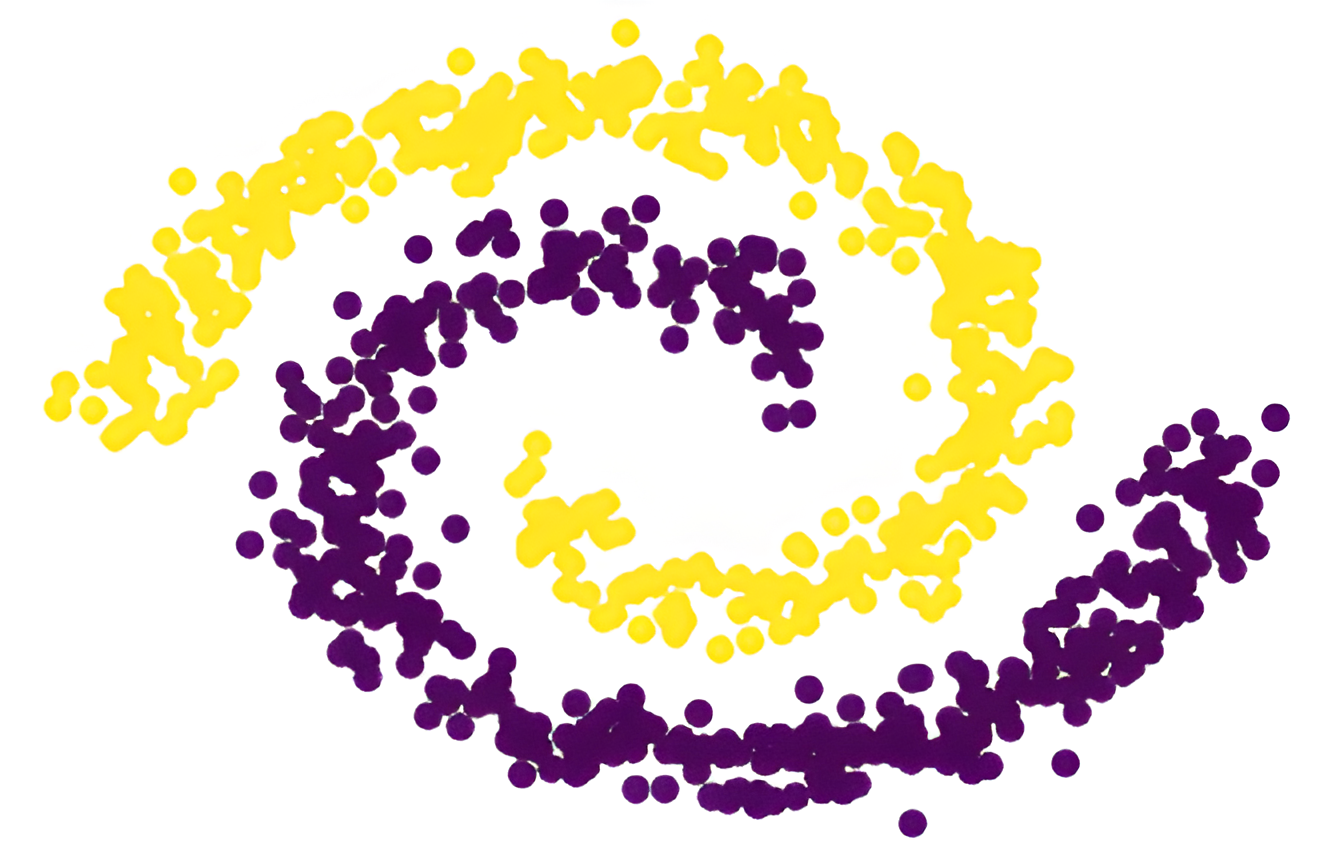
\includegraphics[width=\linewidth]{images/before}}
            \end{figure}
            \column{0.1\textwidth}
            \LARGE
            \[\mathbf{=}\]
            \column{0.27\textwidth}
            \begin{figure}
                \centering
                \fbox{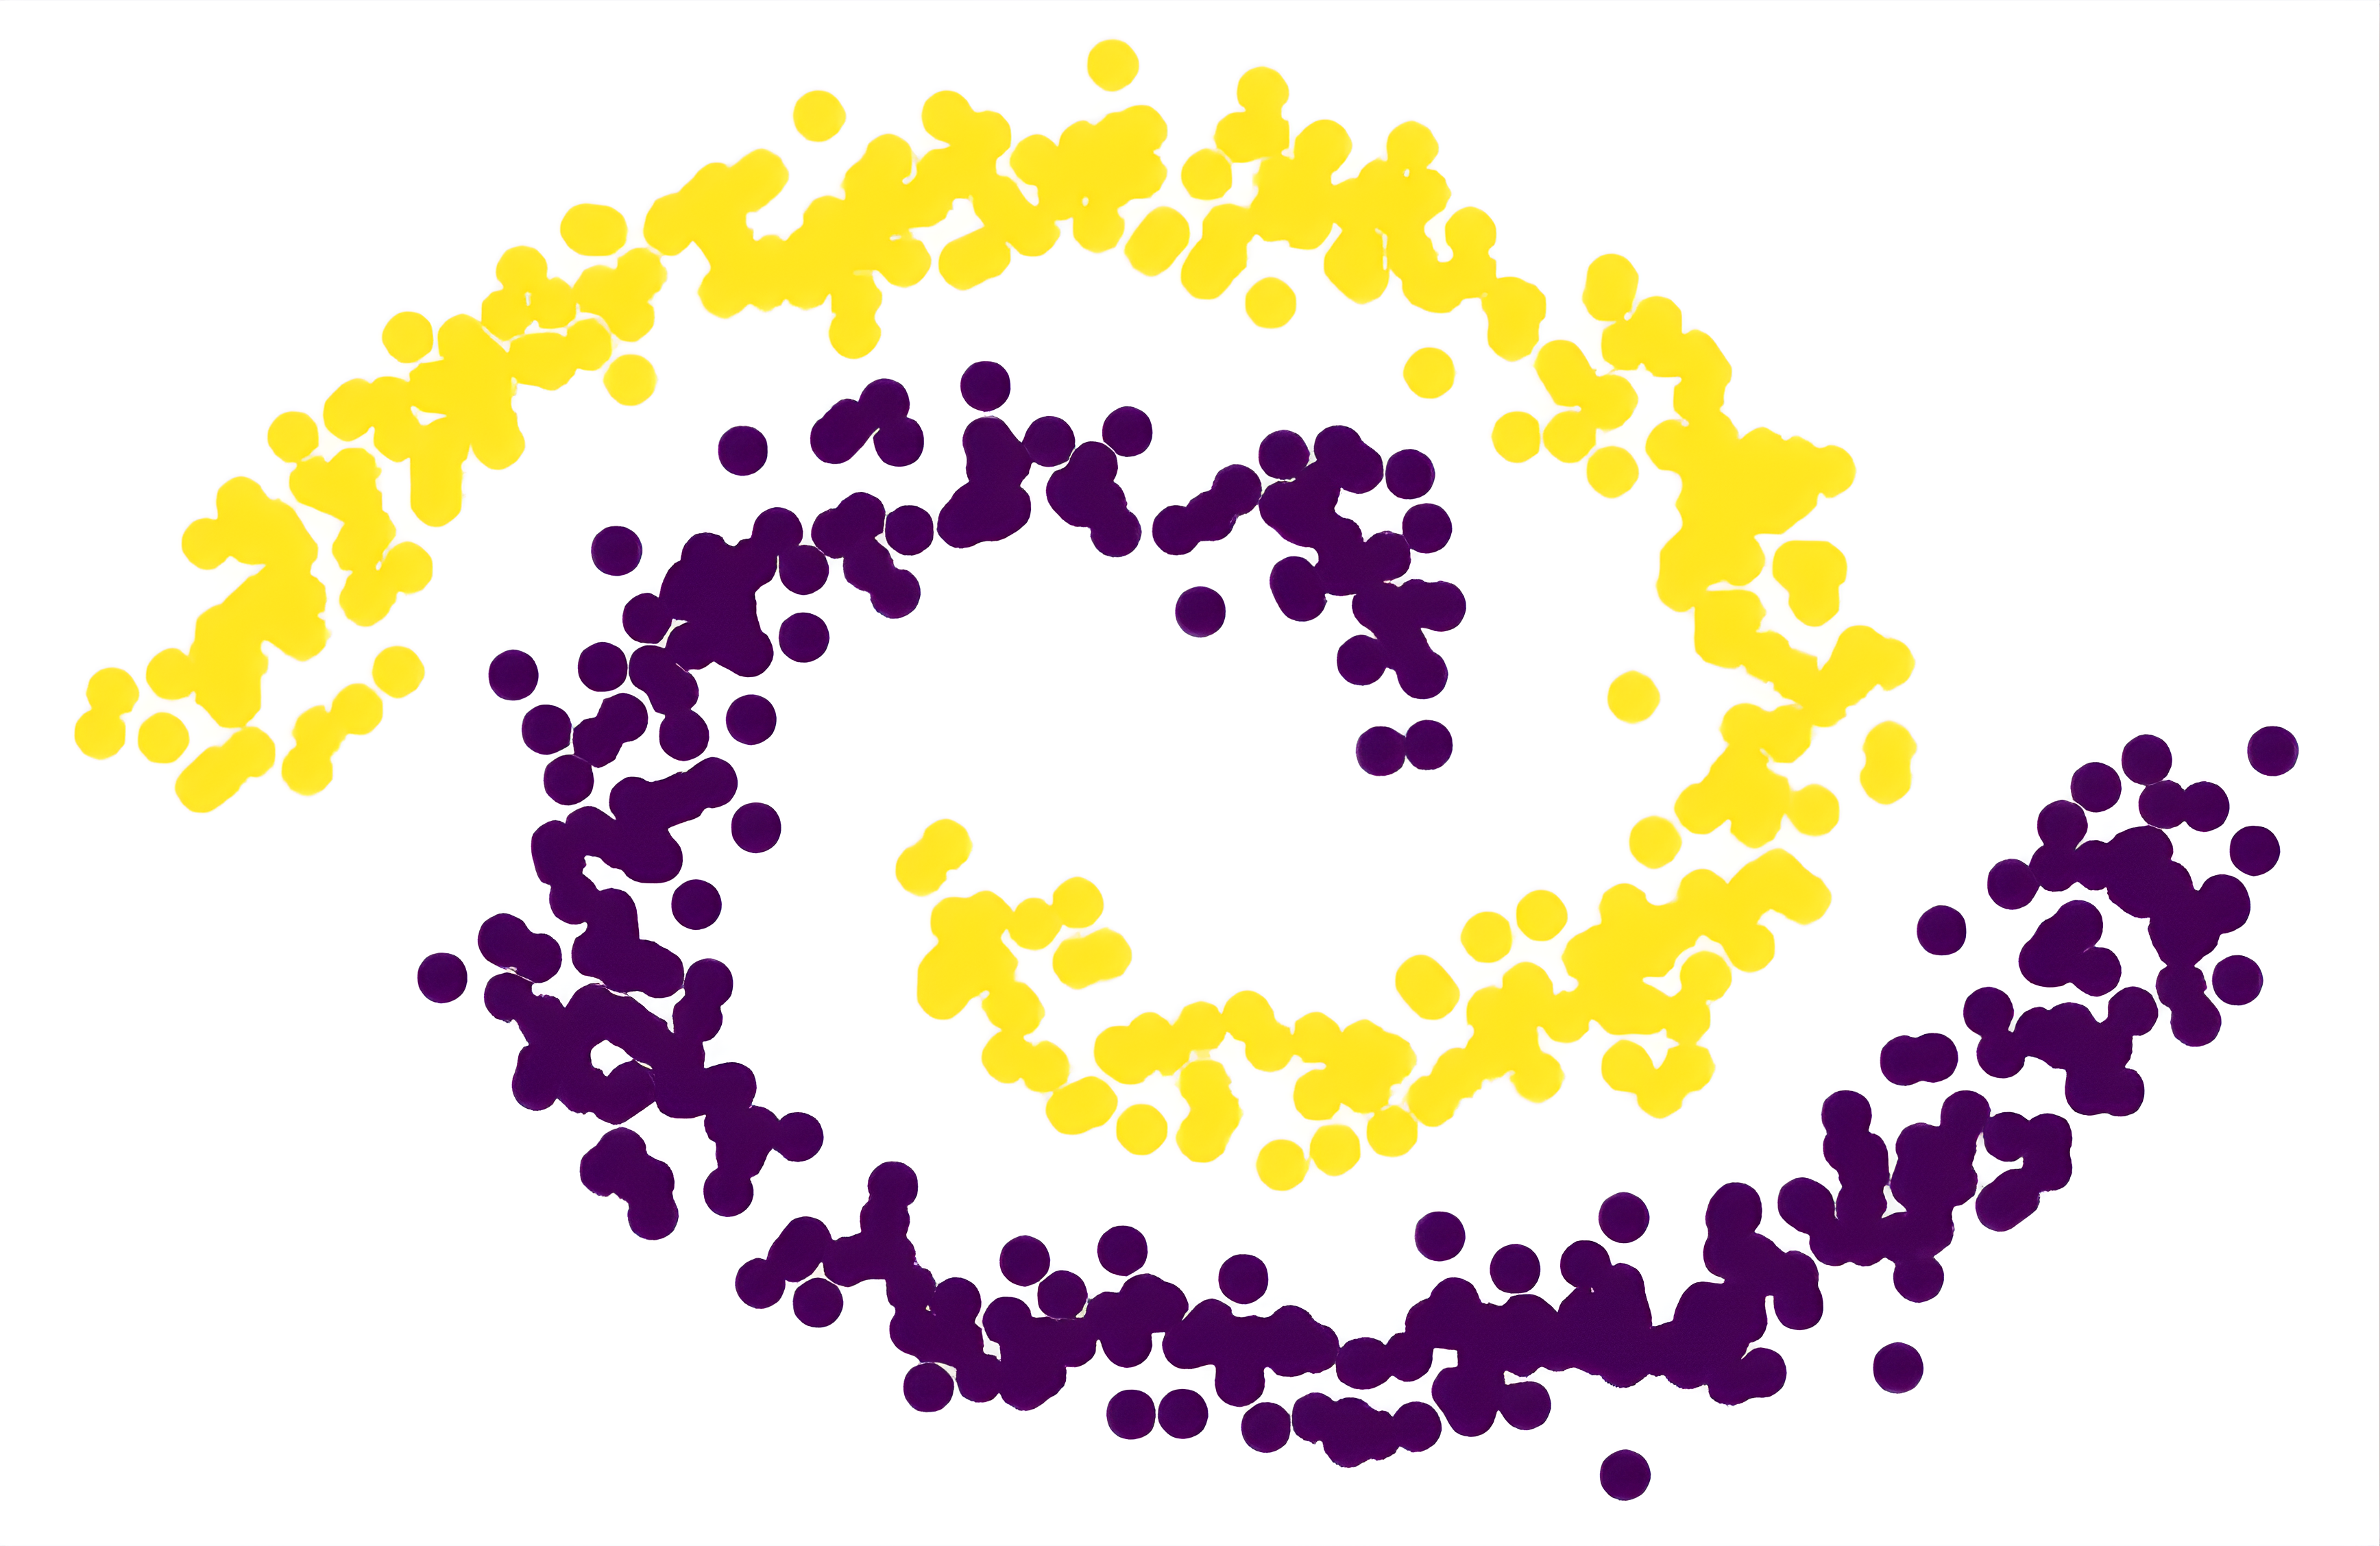
\includegraphics[width=\linewidth]{images/train}}
            \end{figure}
            \column{0.1\textwidth}
            \LARGE
            \[\mathbf{+}\]
            \column{0.27\textwidth}
            \begin{figure}
                \centering
                \fbox{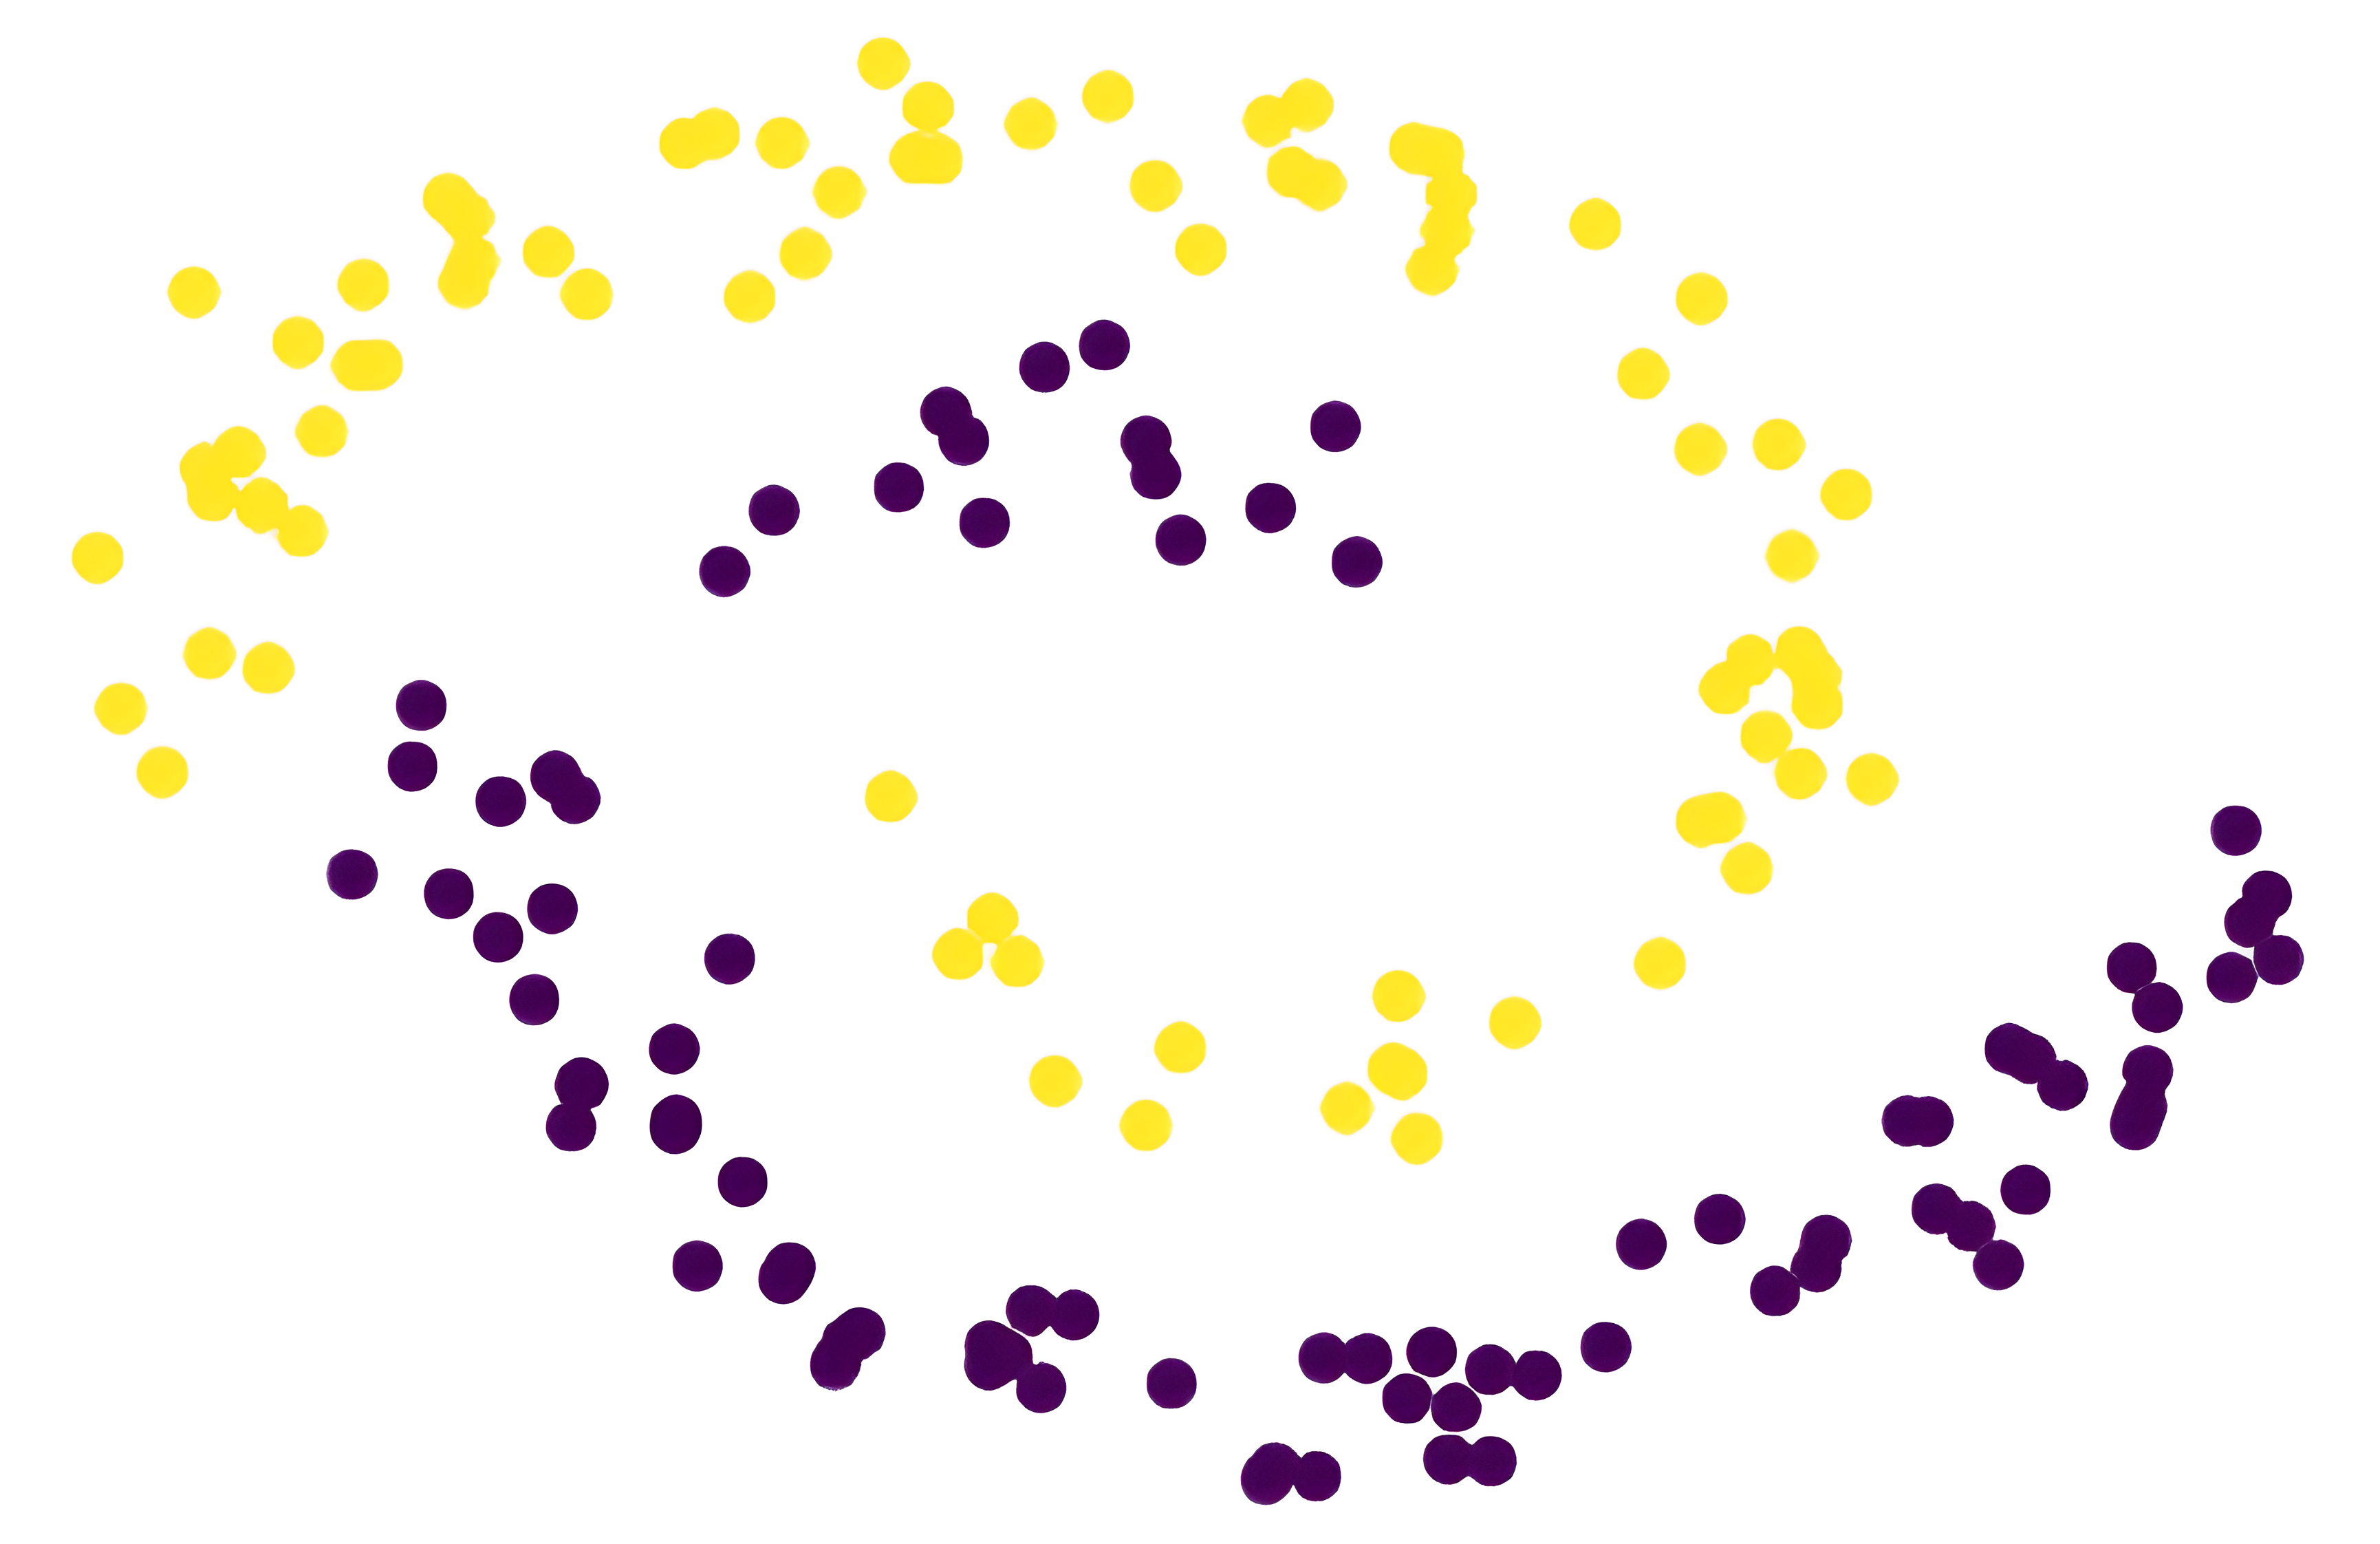
\includegraphics[width=\linewidth]{images/test}}
            \end{figure}
        \end{columns}
        \medskip
        \begin{columns}[onlytextwidth]
            \small
            \column{0.27\textwidth}
            \column{0.1\textwidth}
            \column{0.27\textwidth}
            \centering
            Train
            \column{0.1\textwidth}
            \column{0.27\textwidth}
            \centering
            Test
        \end{columns}

        \vfill

        \begin{columns}[onlytextwidth]
            \column{0.3\linewidth}
            \tiny
            \begin{verbatim}
> linear = svm.SVC(kernel='linear', C=1000)
> linear = model.fit(X_train, y_train)

> poly = …
> rbf = …
            \end{verbatim}
            \column{0.3\linewidth}
            \scriptsize
            \centering
            Soft margin constraints\\
            \frac{1}{2}\mathbf{w}^T\mathbf{w} + \text{C} \sum_{n=1}^{N} \zeta_n
        \end{columns}
    \end{frame}

    \begin{frame}[fragile]{Results and Interpretation}
        \bigskip
        \bigskip
        \begin{columns}[onlytextwidth]
            \scriptsize
            \column{0.33\textwidth}
            \centering
            \begin{figure}
                \centering
                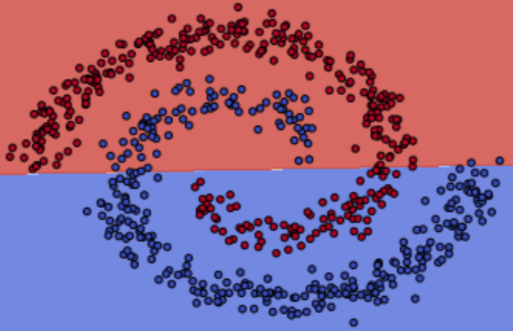
\includegraphics[width=\linewidth]{image-20220624192228376}
                \caption{Linear}
            \end{figure}
            \[K(\mathbf{x}, \mathbf{x}') = \mathbf{x}^T \mathbf{x}'\]
            \column{0.33\textwidth}
            \centering
            \begin{figure}
                \centering
                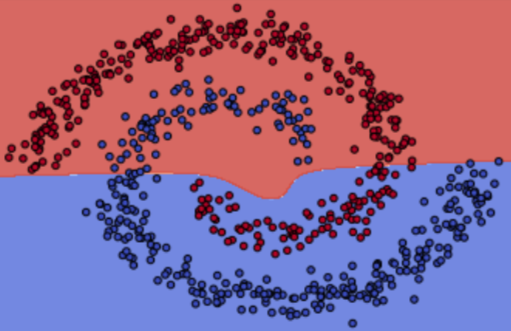
\includegraphics[width=\linewidth]{image-20220624192244841}
                \caption{Polynomial}
            \end{figure}
            \[K(\mathbf{x}, \mathbf{x}')=(1 + \gamma (\mathbf{x}^T\mathbf{x}'))^Q\]
            \column{0.33\textwidth}
            \centering
            \begin{figure}
                \centering
                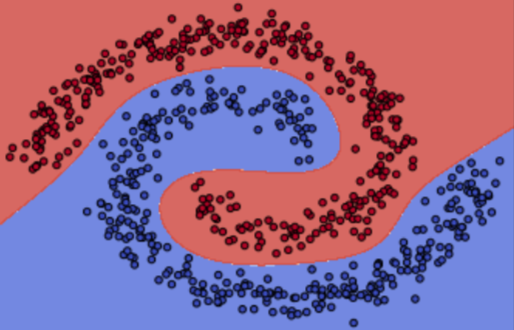
\includegraphics[width=\linewidth]{image-20220624192258535}
                \caption{RBF}
            \end{figure}
            \[K(\mathbf{x}, \mathbf{x}') = e^{-\gamma \mid\mid \mathbf{x}-\mathbf{x}' \mid\mid^2}\]
        \end{columns}

        \bigskip
        \bigskip

        \scriptsize
        \begin{verbatim}
            Q = 3
            gamma = 1 / ({N_train} * X_train.var())
        \end{verbatim}
    \end{frame}

    \begin{frame}[fragile]{Results and Interpretation}
        \bigskip
        \bigskip
        \begin{columns}[onlytextwidth]
            \scriptsize
            \column{0.33\textwidth}
            \centering
            \begin{figure}
                \centering
                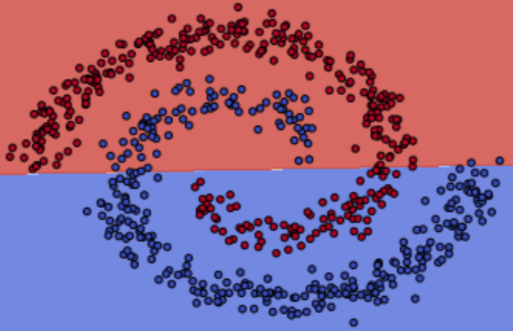
\includegraphics[width=\linewidth]{image-20220624192228376}
                \caption{Linear}
            \end{figure}
            \column{0.33\textwidth}
            \centering
            \begin{figure}
                \centering
                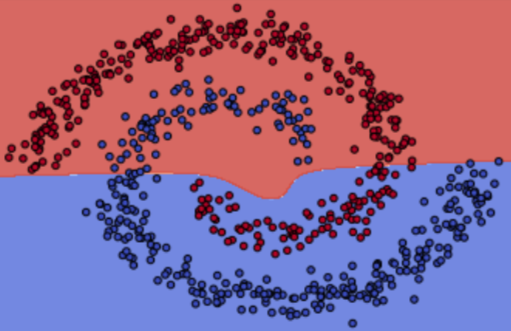
\includegraphics[width=\linewidth]{image-20220624192244841}
                \caption{Polynomial}
            \end{figure}
            \column{0.33\textwidth}
            \centering
            \begin{figure}
                \centering
                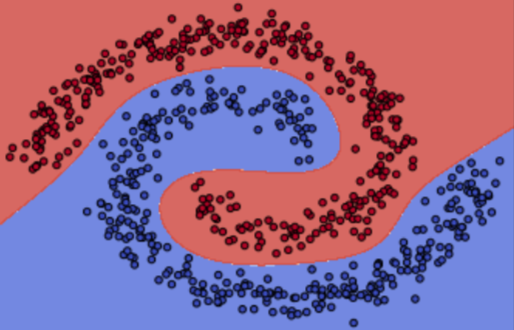
\includegraphics[width=\linewidth]{image-20220624192258535}
                \caption{RBF}
            \end{figure}
        \end{columns}

        \bigskip
        \bigskip

        \centering
        \small
        \begin{itemize}
            \item Difference in the flexibility between the three kernels
            \item Only RBF can replicate the spiral shape
        \end{itemize}
    \end{frame}
    \begin{frame}[fragile]{Polynomial Kernel: different degrees of freedom}
        \begin{columns}[onlytextwidth]
            \scriptsize
            \column{0.33\textwidth}
            \centering
            \begin{figure}
                \centering
                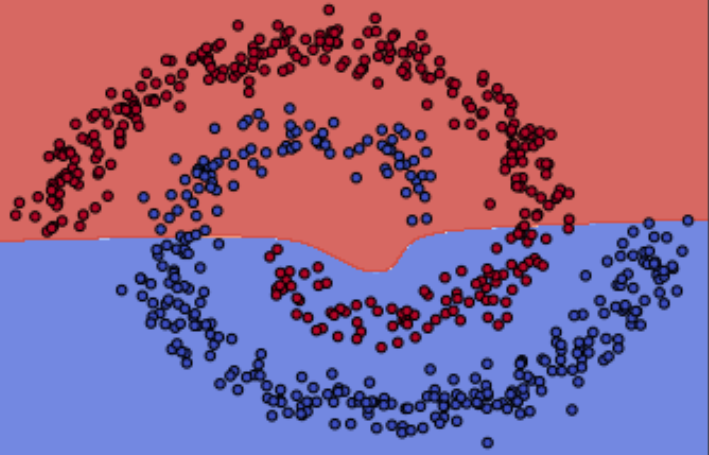
\includegraphics[width=\linewidth]{images/3}
                \caption{3 degr.}
            \end{figure}
            \column{0.33\textwidth}
            \centering
            \begin{figure}
                \centering
                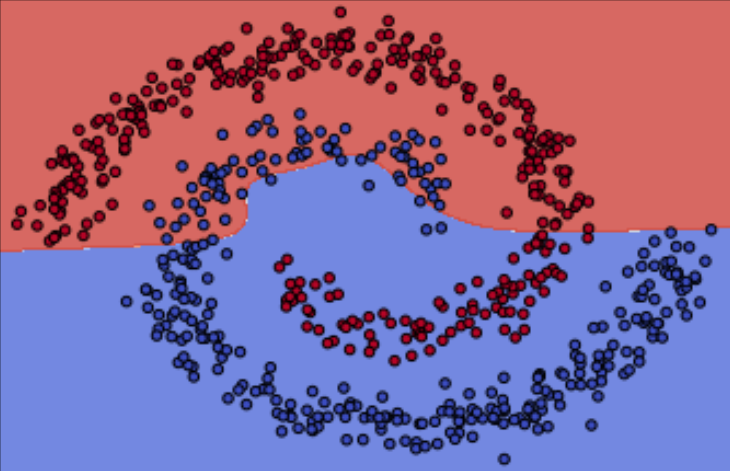
\includegraphics[width=\linewidth]{images/5}
                \caption{5 degr.}
            \end{figure}
            \column{0.33\textwidth}
            \centering
            \begin{figure}
                \centering
                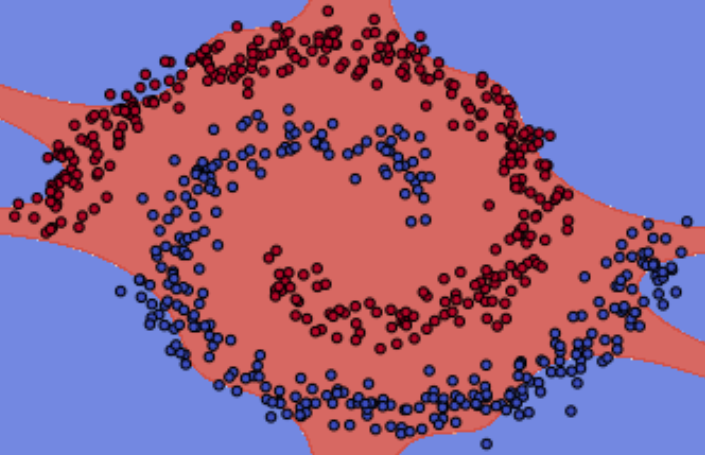
\includegraphics[width=\linewidth]{images/10}
                \caption{10 degr.}
            \end{figure}
        \end{columns}
        \begin{columns}[onlytextwidth]
            \scriptsize
            \column{0.33\textwidth}
            \centering
            \begin{figure}
                \centering
                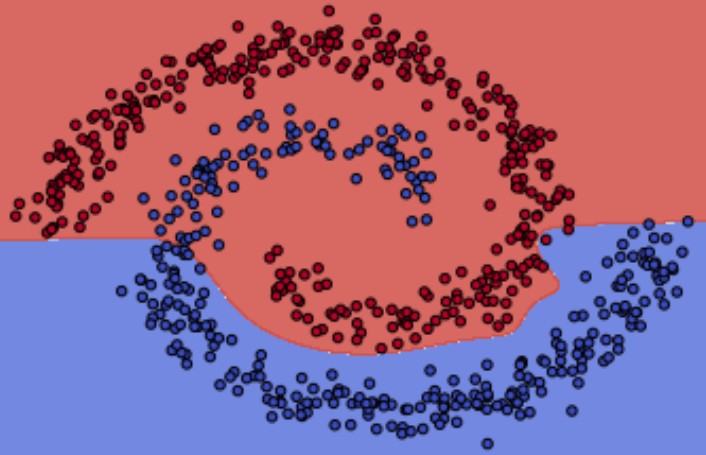
\includegraphics[width=\linewidth]{images/15}
                \caption{15 degr.}
            \end{figure}
            \column{0.33\textwidth}
            \centering
            \begin{figure}
                \centering
                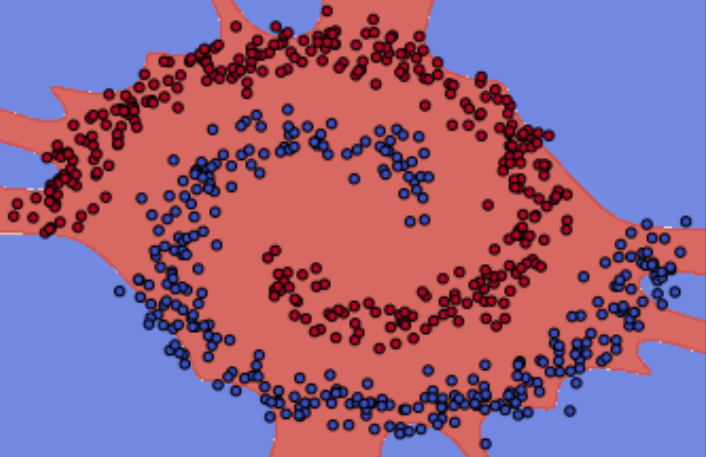
\includegraphics[width=\linewidth]{images/20}
                \caption{20 degr.}
            \end{figure}
            \column{0.33\textwidth}
            \centering
            \begin{figure}
                \centering
                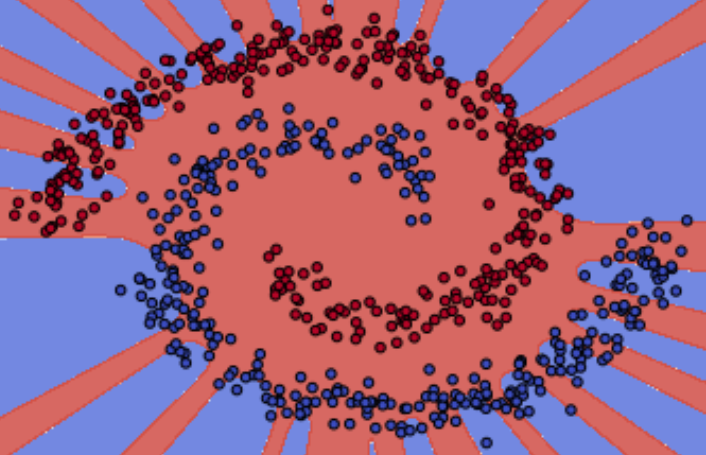
\includegraphics[width=\linewidth]{images/30}
                \caption{30 degr.}
            \end{figure}
        \end{columns}
    \end{frame}


    \begin{frame}{Conclusion}
        \bigskip
        \bigskip
        \begin{columns}[onlytextwidth]
            \scriptsize
            \column{0.33\textwidth}
            \centering
            \begin{figure}
                \centering
                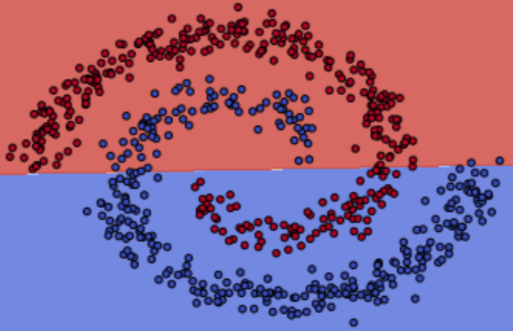
\includegraphics[width=\linewidth]{image-20220624192228376}
                \caption{Linear}
            \end{figure}
            \[E_{\text{test}}^{\text{linear}} = 0.22\]
            #SV’s: 371/800
            \column{0.33\textwidth}
            \centering
            \begin{figure}
                \centering
                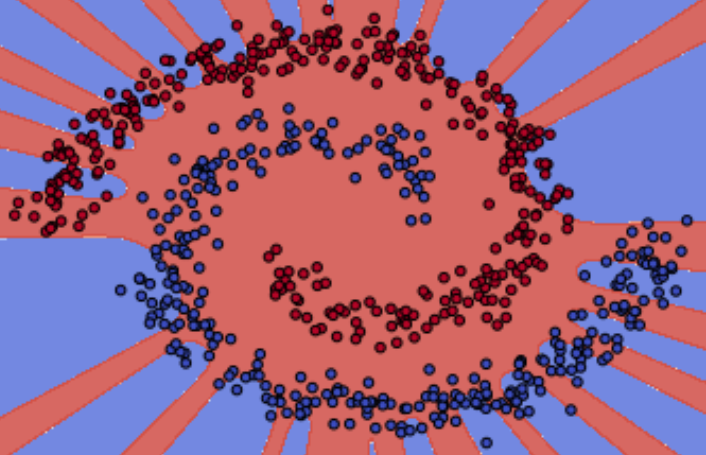
\includegraphics[width=\linewidth]{images/30}
                \caption{Polynomial (30 degr.)}
            \end{figure}
            \[E_{\text{test}}^{\text{poly-30degr}} = 0.54\]
            #SV’s: 492/800
            \column{0.33\textwidth}
            \centering
            \begin{figure}
                \centering
                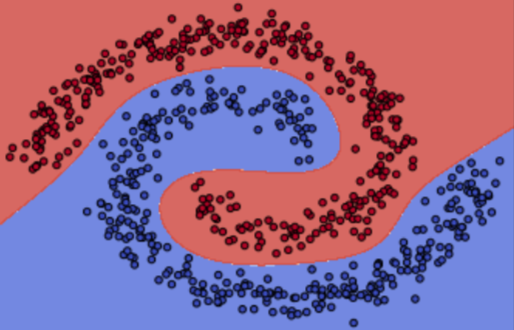
\includegraphics[width=\linewidth]{image-20220624192258535}
                \caption{RBF}
            \end{figure}
            \[E_{\text{test}}^{\text{RBF}} = 0.013\]
            #SV’s: 15/800
        \end{columns}

        \bigskip
        \bigskip

        \small
        \begin{columns}
            \column{0.5\textwidth}
            \begin{block}{RBF}
                \[\mathbb{E}[E_{out}] \le \frac{\mathbb{E}[\text{\# of SVs}]}{\text{N} - 1} = 0.019\]
            \end{block}
        \end{columns}
    \end{frame}


    \section{Decision tree and k-nearest neighbours regressor forecasting}
    \begin{frame}
        \textbf{How does the decision tree regressor model compare to the k-nearest neighbour regressor model in terms of in- and out-of-sample error for time series forecasting?}
    \end{frame}

    \begin{frame}{Decision Tree Regressor}
        \begin{itemize}
            \item Splits data into subsets
            \item Training: searches best features/thresholds to split groups
            \item \textbf{Model = decision tree}
        \end{itemize}
        \begin{columns}[onlytextwidth]
            \column{0.605\textwidth}
            \begin{figure}
                \centering
                \fbox{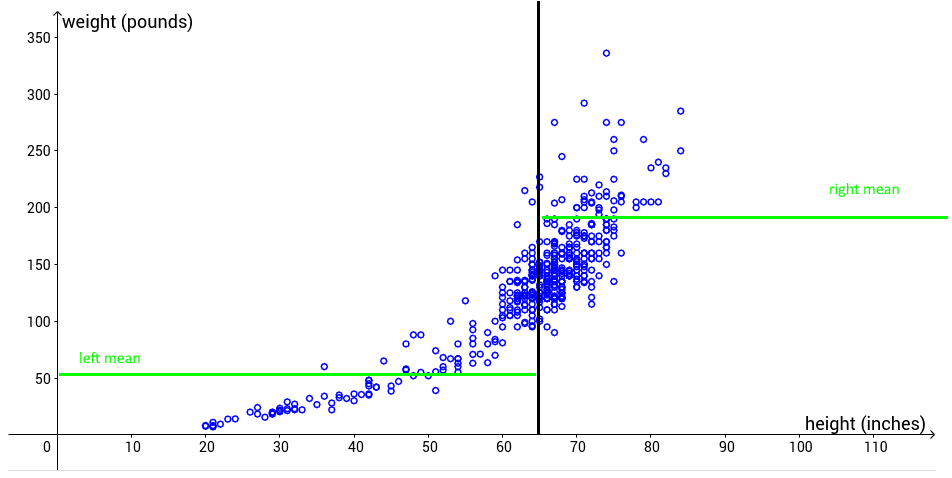
\includegraphics[width=\linewidth]{images/DT1}}
            \end{figure}
            \column{0.35\textwidth}
            \begin{figure}
                \centering
                \fbox{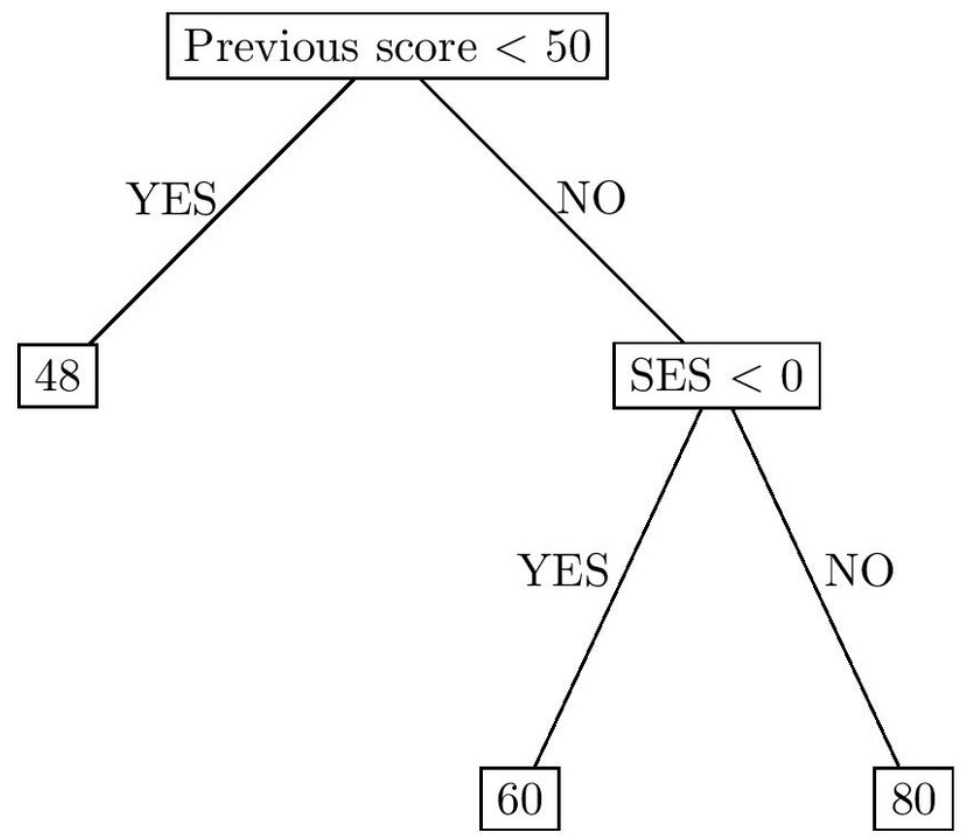
\includegraphics[width=\linewidth]{images/DT2}}
            \end{figure}
        \end{columns}
    \end{frame}

    \begin{frame}{K-Nearest Neighbour Regressor (KNN)}
        \begin{columns}[onlytextwidth]
            \column{0.5\textwidth}
            \begin{itemize}
                \item \textbf{Model = data}
                \item Prediction: mean of target values in neighborhood
            \end{itemize}
            \column{0.45\textwidth}
            \begin{figure}
                \centering
                \fbox{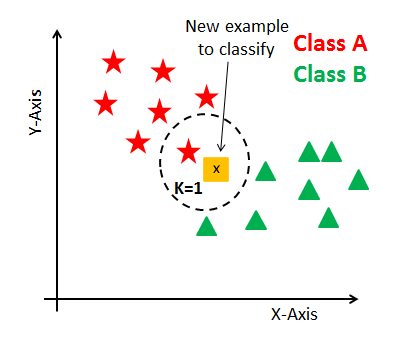
\includegraphics[width=\linewidth]{images/k}}
            \end{figure}
        \end{columns}
    \end{frame}

    \begin{frame}{Dataset}
        \begin{itemize}
            \item \textbf{Given}: temperatures + humidity of specific rooms in the house
            \item \textbf{Objective}: predict Room Humidity in kitchen
            \item Measurement every 10 minutes, for 4 months
        \end{itemize}
        \begin{figure}
            \centering
            \fbox{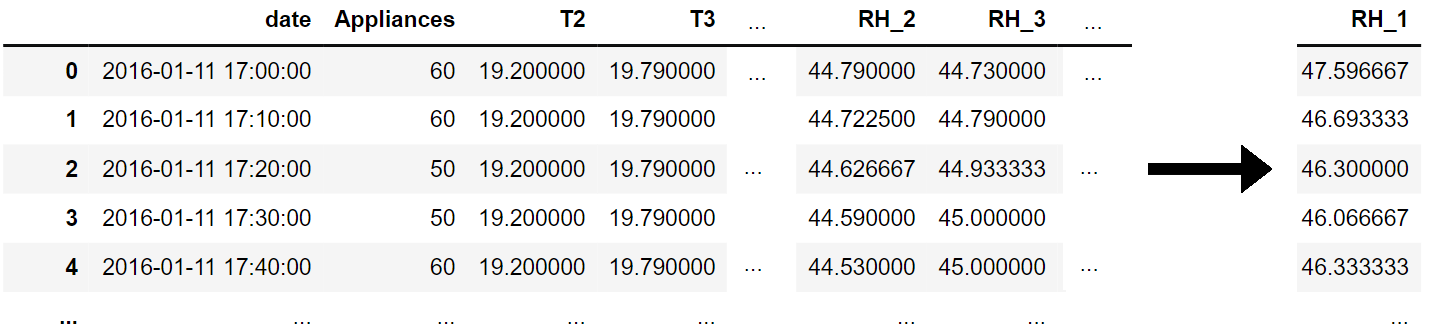
\includegraphics[width=\linewidth]{images/table}}
        \end{figure}
    \end{frame}


    \begin{frame}{Experimental setup}
        \begin{columns}[onlytextwidth]
            \column{0.45\textwidth}
            \centering
            Root-mean-square error:
            \[E = \sqrt{\dfrac{\sum_{n=0}^N (y_n - h(x_n))^2}{N}}\]
            \column{0.45\textwidth}
            \centering
            Regression score:
            \[1-\dfrac{\sum_{n=0}^N (y_n - h(x_n))^2}{\sum_{n=0}^N (y_n - \bar{y})^2}\]
        \end{columns}

        Data:
        \begin{enumerate}
            \item Split into subsequent training and testing set
            \item Process normalised data
        \end{enumerate}

        Model comparison:
        \begin{enumerate}
            \item Baseline models
            \item Equally tuned models through randomised grid search
        \end{enumerate}

    \end{frame}

    \begin{frame}{}
        \bigskip
        \begin{figure}
            \centering
            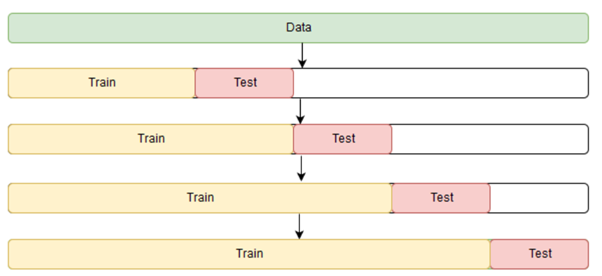
\includegraphics[width=\linewidth]{images/validation}
            \caption{Time series cross-validation for forecasting}
        \end{figure}
    \end{frame}

    \begin{frame}{}
        \bigskip
        \begin{figure}
            \centering
            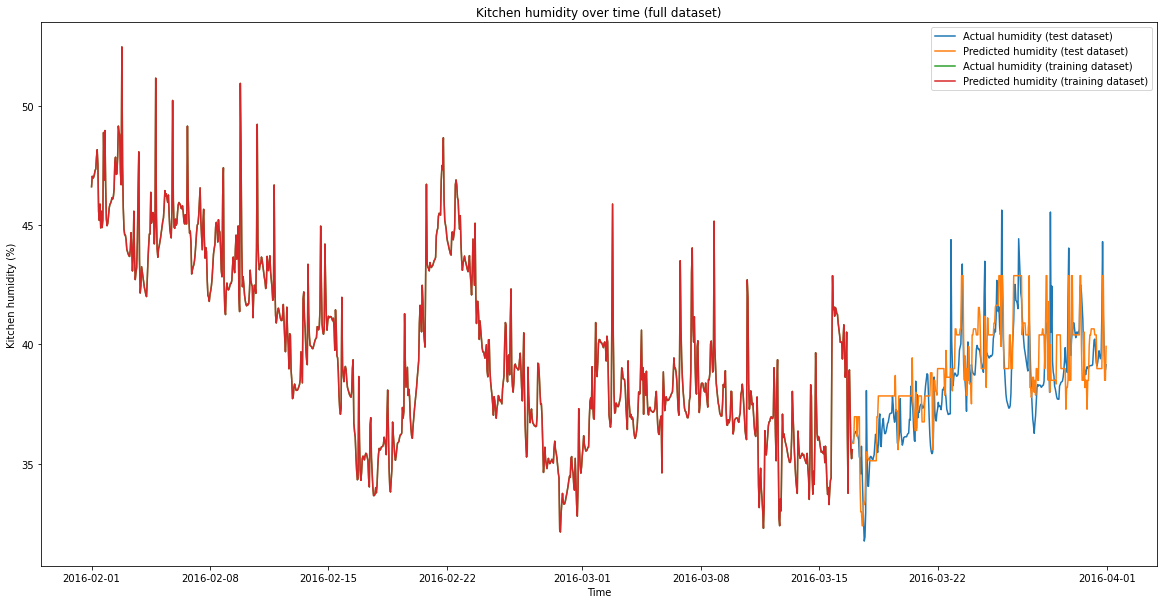
\includegraphics[width=\linewidth]{images/full}
            \caption{Baseline decision tree regressor}
        \end{figure}
    \end{frame}
    \begin{frame}{}
        \bigskip
        \begin{figure}
            \centering
            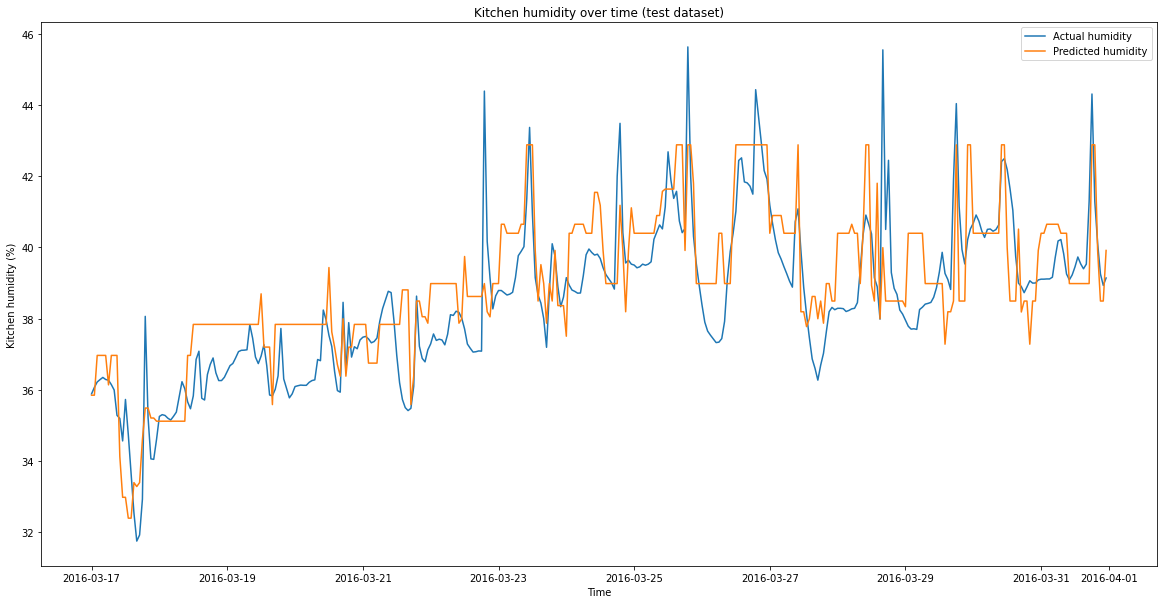
\includegraphics[width=\linewidth]{images/baseline_tree}
            \caption{Baseline decision tree regressor}
        \end{figure}
        \small
        \begin{table}
            \begin{tabular}{l l l}
                & Training & Testing \\
                Score & 1.000    & 0.479   \\
                RMSE  & 0.000    & 1.551
            \end{tabular}
        \end{table}
    \end{frame}
    \begin{frame}{}
        \bigskip
        \begin{figure}
            \centering
            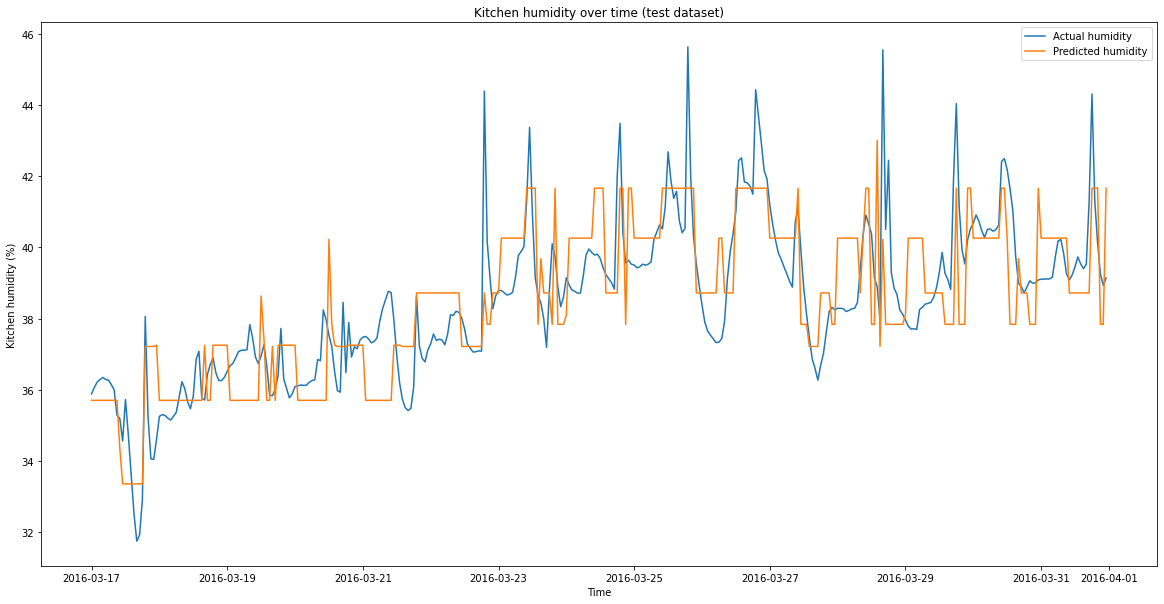
\includegraphics[width=\linewidth]{images/tuned_tree}
            \caption{Tuned decision tree regressor}
        \end{figure}
        \small
        \begin{table}
            \begin{tabular}{l l l}
                & Training & Testing \\
                Score & 0.949    & 0.554   \\
                RMSE  & 0.871    & 1.434
            \end{tabular}
        \end{table}
    \end{frame}
    \begin{frame}{}
        \bigskip
        \begin{figure}
            \centering
            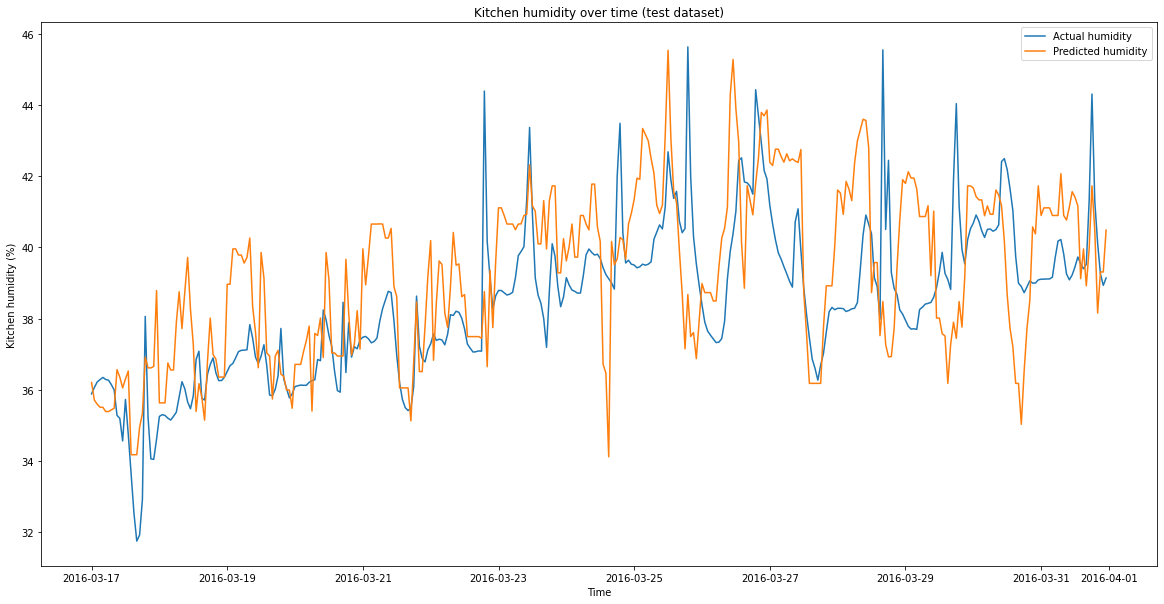
\includegraphics[width=\linewidth]{images/baseline_k}
            \caption{Baseline k-nearest neighbours regressor}
        \end{figure}
        \small
        \begin{table}
            \begin{tabular}{l l l}
                & Training & Testing \\
                Score & 0.945    & 0.040   \\
                RMSE  & 0.908    & 2.105
            \end{tabular}
        \end{table}
    \end{frame}

    \begin{frame}{}
        \bigskip
        \begin{figure}
            \centering
            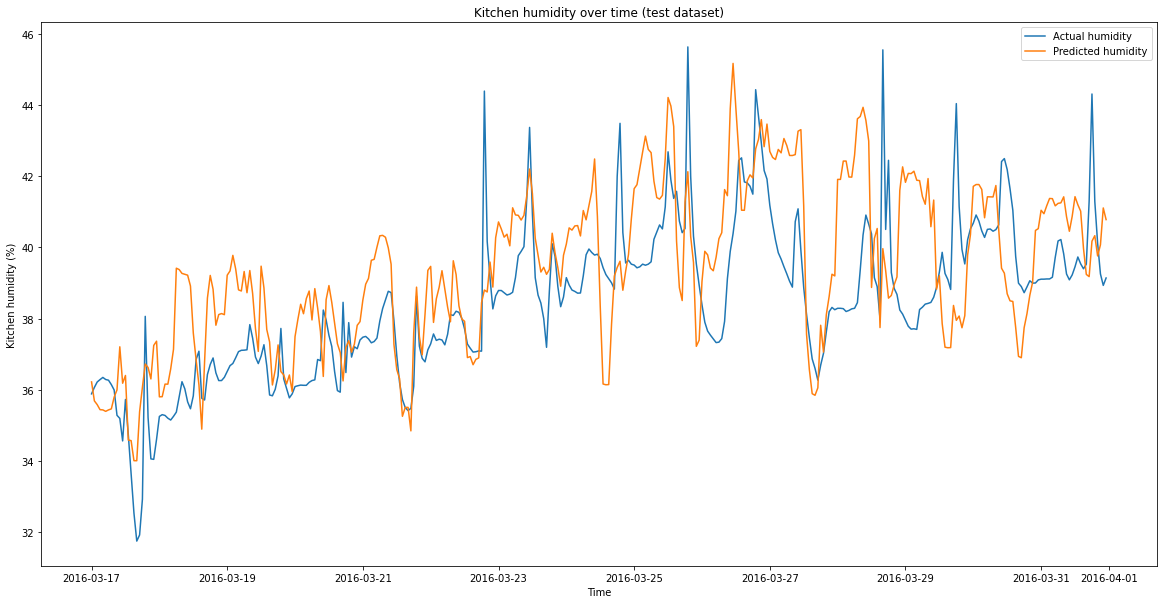
\includegraphics[width=\linewidth]{images/tuned_k}
            \caption{Tuned k-nearest neighbours regressor}
        \end{figure}
        \small
        \begin{table}
            \begin{tabular}{l l l}
                & Training & Testing \\
                Score & 1.000    & 0.089   \\
                RMSE  & 0.000    & 2.050
            \end{tabular}
        \end{table}
    \end{frame}

    \begin{frame}{Conclusions}
        \begin{itemize}
            \item Tuned decision tree regressor is most likely to generalise best

            \item Model nature is visible in predictions:
            \begin{itemize}
                \item[-] Decision tree predicts conservative smooth surfaces
                \item[-] K-nearest neighbours predicts noisy erratic changes resembling the training data
            \end{itemize}

            \item Time-series forecasting is extrapolation

            \item Model selection can improve $E_{out}$ by reducing or increasing model complexity

            \item Data preprocessing and feature selection is important and can be guided also by cross-validation
        \end{itemize}
    \end{frame}

\end{document}
